\section{Experimental Design}
\label{sec:methodology}

\subsection{RQ1: Identification of SUIT Smells}
\label{sec:experience-design-smells-collection}
%
\begin{figure}
\centering
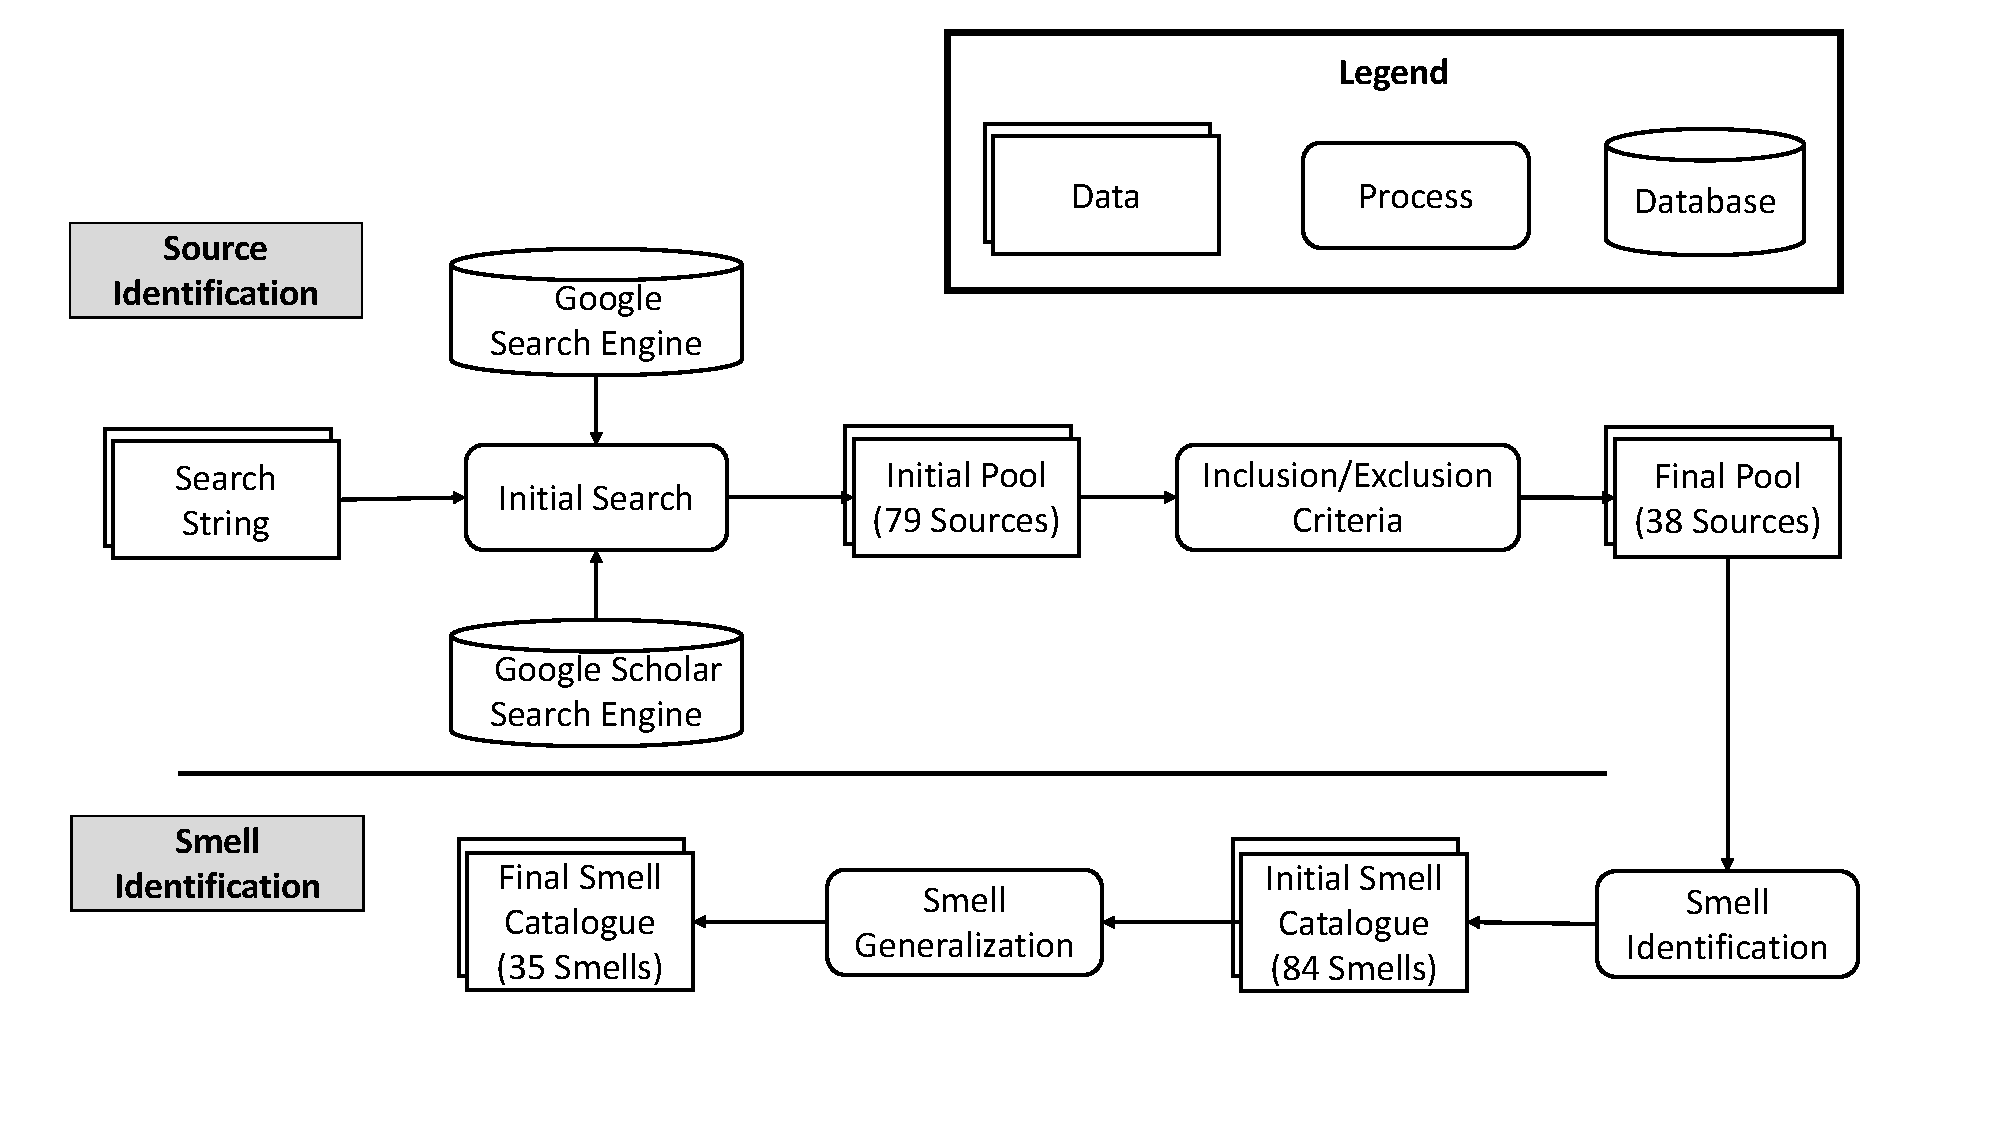
\includegraphics[width=\linewidth]{figures/smells/smell-catalgogue-process.pdf}
\caption{Overview of the process to establish the SUIT smell catalog.}  
\label{fig:smell-catalog-process}
\end{figure}

To perform a study on the impact of smells in SUITs, we first need to build a reliable and representative catalog of test smells. To this end, we start our investigation by collecting SUIT smells presented in both academic and grey literature. 
We classify in the academic or white literature papers that are published in peer-reviewed conferences or journals. On the other hand, we classify as grey literature white-papers, magazines, online blog-post, question-answers sites, survey results, and technical reports following the methodology presented in \textcite{Ricca2021}. Indeed, the grey literature constitutes a rich source of documents where practitioners share their experiences, propose guidelines, or even ask and answer questions. Thus, we conduct a multivocal literature review following the steps depicted by \textcite{Garousi2018}. 
Figure~\ref{fig:smell-catalog-process} summarizes our adoption of these steps in the process of building a catalog of SUIT smells.

\paragraph{\textbf{Initial Search.}}

To mine the academic sources we rely on the Google Scholar Search engine, whereas for the grey literature we rely on the Google Search engine. These two search engines are known to subsume other databases and repositories that \cite{Garousi2018}, hence, we limit our investigation to these two search engines. We compile a list of search terms such as ``acceptance test'', ``test automation'', ``end-to-end test'', ``system test'' and ``behavior test'' to define the type of tests that we are targeting and combine those strings with each of the following: ``smell'', ``symptom'', ``anti pattern'' and ``bad practice''. This allows to generate the following search string for the engines: \emph{software and ("acceptance test" OR "test automation" OR "end-to-end test" OR "system test" OR "functional test") AND ("smell" OR "symptom" OR "anti pattern" OR "bad practice")}. To validate the search string we run it and make sure that relevant documents known \emph{a priori} appear in the results \cite{Kitchenham2007, Ricca2021}. 
%Shall we mention this document
Then, we proceed to a systematic review of all the sources in order to identify test smells. However, because the search string returns about 1,370,000 results in the Google Search Engine and about 12,100 results in the Google Scholar Search Engine, we restrict our analysis to an initial pool composed of the first 200 results in each engine, at which point the number of relevant sources per page drops to zero. From those, we read the title and abstract available to decide whether or not to further analyze the articles. This leads to a initial list composed of 47 sources in the grey literature and 32 sources in the academic literature for a total of 79 sources.

\paragraph{\textbf{Inclusion/Exclusion Criteria.}}

To be eligible for our study, a smell must address the code of a SUIT. However, the terms adopted in both industry and academia might not refer to how the test interacts with the application, but rather to what is the intent of the test (\emph{e.g.} acceptance testing) or its scope (\emph{e.g.} system test). This leads to a series of sources discussing tests that are not SUITs and are not compatible with them, typically, white-box tests. Furthermore, some sources address testing issues that are not related to the code base such as organizational smells, which are outside the scope of this study. Indeed, some smells do not target the test code but testers' behavior, \emph{e.g.} \emph{Making Intermittent Bugs Low Priority} \cite{StackExchange2017} for which bugs making the functional test suite fail intermittently at low intervals are ignored. By excluding these irrelevant sources, we reduce our list to 32 sources from the grey literature and 6 sources in the academic literature for a total of 38 sources. The drastic drop in the academic literature is due to the large number of studies targeting unit tests instead of SUITs.
The selection process is depicted in the summary sheet\footnote{Available as \href{https://docs.google.com/spreadsheets/d/e/2PACX-1vQ78jmOjU3qTOlGzwCSkidJOliPKNDQhmuOxSsfTaRqFVjmFP41JUbYQeupqU_lGCK6L4EpQ3FHNGhU/pubhtml}{a spreadsheet}}.

\paragraph{\textbf{Smell Identification.}}

Relying on this final pool of sources, where each source contains at least one SUIT smell, we proceed to the smell identification where we filter out all the smells that are not suitable for our analysis. Indeed, some smells are not applicable to the framework under study \emph{e.g.}, \emph{Dependence on Record and Playback} \cite{StackExchange2017} in which tests are created using Record and Playback, a feature that is not supported by Robot Framework. Other smells are too technology-specific \emph{e.g.}, not using the page object pattern in Selenium tests \cite{Advolodkin2018}. The outcome of this process is an initial smell catalog of 84 unique SUIT smells for which we can derive a metric by analyzing the code representing the symptom observed.

\paragraph{\textbf{Smell Generalization.}}
%Is generalization the best term here? 
Some SUIT smells gathered in the previous step exhibit large overlaps; thus, we proceed to a smell generalization step. For instance, the smell \emph{Enter Enter Click Click} \cite{Buwalda2015} is grouped with \emph{Comments and documentation instead of abstraction} \cite{Klarck2014}, since both smells target the presence of low level actions in the acceptance criteria but in the latter a specific emphasis is put on the documentation aspect. Consequently, we consider those two smells to present similar symptoms and effects and we group them in one smell named \emph{Lack of encapsulation} \cite{Chen2012, Klarck2014, Buwalda2015, England2016, Renaudin2016}. Finally, we observe that some test smells are subsuming others. This is the case for the smells \emph{Hardcoded Values} and \emph{Using condition in test logic} that are both subsumed by the definition of \emph{Obscure test} \cite{Hauptmann2013, Gawinecki2016, Siminiuc2019}. In this example we only keep the latter.  Finally, from this list, we filter out any test smell that would require the test to be executed in order to be observed. As a result, the outcome of this step is a catalog of 35 SUIT smells\footnote{Available at https://github.com/UL-SnT-Serval/suit-smell-catalog} that can be detected statically.

Finally, conducting our study using Robot Framework, we exclude four test smells that cannot be observed in this specific language and its associated framework. Furthermore, we omit 15 test smells because, despite our best efforts, no straightforward metric, avoiding false positives, could be constructed by analyzing the test code. Hence, in this work, we present a list of 16 SUIT smells. A comprehensive description of each smell is presented in Section~\ref{sec:results-smells-collection}.

\subsection{Dataset}
\label{sec:data-collection}
To answer RQ2 and RQ3, we conduct a case study on 13 test suites written in Robot Framework. We establish two sets of projects: the first set is composed of 48 repositories from our partner site, BGL BNP Paribas, and the second set of projects is composed of 12 open-source projects mined from Github. Table~\ref{tab:projects} summarizes the overall properties of these projects. In the following, we describe the projects and present the collection process. 

\subsubsection{Industrial project:}
We leverage the codebase of our industrial partner, BGL BNP Paribas. Where the empirical analysis from Chapter~\ref{chap:evolution-system-user-interactive-test} focuses on the test suite for one project, \emph{SubjectA}, in this chapter, the entire test suite is considered. This test suite targets desktop, web, and mobile applications that are depending on services developed following a service-oriented architecture (SOA). For instance, BGL BNP Paribas developed internal services using Java Swing which rely on either the \gls{api} exposed by the Swing development or rely on computer vision, through the use of the Sikuli\footnote{http://sikulix.com/} library. BGL BNP Paribas also use the Robot Framework to test its mobile client application relying on the Appium\footnote{https://appium.io/} Library.

The goal of the team is to assess compliance to functional requirements by conducting acceptance testing. Today, the test suite consists of 559 tests stored across 48 repositories on an on-premise GitLab instance. While some repositories are defining \emph{Test Cases}, others are used as resources of common \emph{Keywords} where a series of generic \emph{Keywords} specific to the BGL BNP Paribas architecture have been created to help with the development effort as well as to avoid code duplication. A typical example is a login to the ecosystem which is common to a large number of services, and consequently can be mutualized. Hence, in this study, we merge all the repositories to count them as one project, which explains the larger number of \emph{User Keywords} observed in Table~\ref{tab:projects} for the project \emph{bgl}.

\subsubsection{Open-source projects:} 
To collect the open-source test suites, we use the Github Search \gls{api} to mine repositories containing suitable test suites, \ie\ Robot Framework test suites interacting with the \gls{sut} through its user interface. From the results of this first step, we filter out toy projects and tutorials, projects using Robot Framework for its robot process automation capabilities in production, and libraries extending the capabilities of Robot Framework. Following this approach, we gather 23 repositories from Github. Finally, to ensure that maintenance was performed on the test suite itself, we analyze the number of commits involving the Robot Framework test suite for each project, \emph{i.e.} SUIT modifying commit, and discard any project with less than 100 SUIT modifying commits. This process yields a total of 12 repositories presented in Table~\ref{tab:projects}.

The data collection process leads to a total of 2,884,383 \gls{suit}s analyzed across all the versions of all the projects where 2,742,271 originate from the open-source projects and 142,112 from the industrial projects gathered at BGL BNP Paribas. Among those tests, the majority both in industrial and in open-source projects target web applications. The \gls{suit}s interact with such applications through their webpages by interacting with the \gls{dom} or by relying on computer vision to isolate GUI elements. Some operations generate emails or reports, thus, some tests rely on operating system interaction to check that an email was properly sent through a mail client or assess the existence and parses the content of a generated PDF documents.

\begin{table}
\centering

\caption{Metrics for the 13 projects under study. \emph{LoC} is the number of lines of Robot Framework Code, \emph{\#Commits} is the number of commits implicating Robot Framework code, and \emph{\#TestCases} and \emph{\#Keywords} are the number of test cases and user keywords respectively in the last commit of the projects.}
\label{tab:projects}

\begin{tabular}{>{\raggedright}p{0.9in}>{\raggedleft}p{0.7in}>{\raggedleft}p{0.7in}>{\raggedleft}p{0.7in}>{\raggedleft}p{0.7in}}

\toprule
\scriptsize{\textbf{Name}} & \scriptsize{\textbf{LoC}} & \scriptsize{\textbf{\#Commits}} & \scriptsize{\textbf{\#TestCases}} & \scriptsize{\textbf{\#Keywords}} \tabularnewline
\toprule

\scriptsize{\textbf{bgl}} & \scriptsize{57,030} & \scriptsize{309} & \scriptsize{559} & \scriptsize{5,000} \tabularnewline

\midrule

\scriptsize{\textbf{apinf}} & \scriptsize{1,068} & \scriptsize{345} & \scriptsize{74} & \scriptsize{138} \tabularnewline
\scriptsize{\textbf{bikalims}} & \scriptsize{4,446} & \scriptsize{1,279} & \scriptsize{76} & \scriptsize{172} \tabularnewline
\scriptsize{\textbf{collective-cover}} & \scriptsize{1,317} & \scriptsize{943} & \scriptsize{24} & \scriptsize{31} \tabularnewline
\scriptsize{\textbf{cumulus-ci}} & \scriptsize{1,599} & \scriptsize{1,429} & \scriptsize{132} & \scriptsize{34} \tabularnewline
\scriptsize{\textbf{harbor}} & \scriptsize{7,270} & \scriptsize{3,131} & \scriptsize{246} & \scriptsize{472} \tabularnewline
\scriptsize{\textbf{ifs}} & \scriptsize{8,466} & \scriptsize{5,606} & \scriptsize{494} & \scriptsize{605} \tabularnewline
\scriptsize{\textbf{mms-alfresco}} & \scriptsize{1,797} & \scriptsize{504} & \scriptsize{156} & \scriptsize{8} \tabularnewline
\scriptsize{\textbf{mystamps}} & \scriptsize{2,361} & \scriptsize{353} & \scriptsize{212} & \scriptsize{111} \tabularnewline
\scriptsize{\textbf{ozone}} & \scriptsize{2,636} & \scriptsize{271} & \scriptsize{230} & \scriptsize{90} \tabularnewline
\scriptsize{\textbf{plone}} & \scriptsize{1,046} & \scriptsize{211} & \scriptsize{59} & \scriptsize{163} \tabularnewline
\scriptsize{\textbf{plone-intranet}} & \scriptsize{2,225} & \scriptsize{1,759} & \scriptsize{213} & \scriptsize{134} \tabularnewline
\scriptsize{\textbf{rspamd}} & \scriptsize{3,397} & \scriptsize{685} & \scriptsize{429} & \scriptsize{151} \tabularnewline

\bottomrule

\end{tabular}

\end{table}

To conclude this section, we observe that the dataset is composed of projects covering various domains, technology stacks, sizes for both industrial and open-source projects. Thus, we believe that this diversity allows avoiding biases observed in one type of project and improves the generalization of the observations.

\subsection{RQ2: SUIT Smells Distribution}
\label{sec:smell-detection}

For each of the SUIT smells that we gathered, we compute a metric to automatically measure a smelliness score for the affected test. We rely on heuristics to construct these metrics. To this end, we apply the high-level investigation mechanism framed by \textcite{Marinescu2004} called ``detection strategy''. As defined by the author, a ``detection strategy'' is \emph{a generic mechanism for analyzing a source code model using metrics}. The detection strategies are formulated in a series of steps: (1) Break-down informal rules into symptoms that can be captured by a single metric; (2) Select a proper set of metrics to quantify each of the symptoms; (3) Define thresholds that classify a test as smelly or not; (4) Use operators to associate the symptoms leading to the final rule for detecting the smells.

Note that step 3 of this approach describes the definition of a threshold. Even though different approaches have been proposed, \emph{e.g.} using semantical properties and statistical distributions \cite{Marinescu2004} or using Bayesian belief networks \cite{Khomh2009}, defining a good threshold remains a hard and error-prone task. Thus, more recently, researchers have been trying to avoid this limitation by using machine learning to directly learn what a smell looks like avoiding altogether the use of a threshold \cite{ArcelliFontana2016}. In this work, in order to avoid any bias generated by a binary classification, we do not apply any empirical threshold (with the exception of one smell, \emph{Long Test Steps}) but focus our analysis on the observation of the symptoms associated with SUIT smells. Hence, for each test, we attribute a metric that represents the number of symptoms that are observed in a test. Furthermore, we propose a density metric, which normalizes the number of symptoms observed over the worst-case scenario for a given test. Indeed, our goal is to analyze how the symptoms are treated by the maintainers of the test code base and not to classify tests as smelly or not.

To extract code metrics, we rely on a parsing engine presented in Section~\ref{sec:tree-representation-KDT}. The parser generates for each test a call tree, where the root is the entry point of the test and the leaf nodes are the actions generated on the system under test, or the application driver layer if we refer to the three-layer architecture described by \textcite{Humble2010}. Each leaf node is annotated with information such as the type of action (assertion, getter, event, etc.) and each variable can be inferred a type based on the \emph{Library Keywords} calling it. To create the metrics, we rely on heuristics exhibiting the symptom associated with the smell. While building the heuristics, we focus on high precision, even though this might lead to a low recall.

Where the detection of SUIT smells is typically performed using code metrics, in the case of one of the SUIT smells, namely \emph{Using Personal Pronoun}, such metrics are not sufficient. Hence, we rely on natural language processing to extract information about the name of some \emph{Keywords} and use text tagging to define whether or not the subject of the \emph{Keywords} is the first-person pronoun or not.

When computing the metrics, we introduce two types of metrics: a count metric $S$ and a density metric $D$. The count metric $S$ counts the number of instances of a symptom observed in a test. On the other hand, the density metric $D$ provides an indication of the number of instances over a maximum value that could have appeared in the test. Thus, the density metrics vary between 0 and 1, 0 indicating the absence of any of the symptoms, and 1 indicates that for each of the possible locations for the symptom to be present, it appeared in the test.

Finally, to assess the diffusion of the symptoms across the test suite we present the total number of symptomatic tests $\abs{t_s}$ over the total number of tests, $\abs{t}$. Thus $\abs{t_s} / \abs{t}$ measures the percentage of tests presenting an instance of a symptom for a smell $s$. Table~\ref{tab:metrics} presents a summary of all the metrics.

\begin{table}
\centering

\caption{Definitions of the metrics used in the study.}
\label{tab:metrics}

\begin{tabular}{>{\raggedright}p{1.2in}>{\raggedright}p{0.6in}>{\raggedright}p{3in}}

\toprule
\scriptsize{\textbf{Name}} & \scriptsize{\textbf{Notation}} & \scriptsize{\textbf{Description}} \tabularnewline
\toprule

\scriptsize{\# Symptoms} & \scriptsize{$S_s$} & \scriptsize{The number of symptoms for a smell $s$ counted in a single test.} \tabularnewline
\scriptsize{\% Symptoms} & \scriptsize{$D_s$} & \scriptsize{The number of symptoms for a smell $s$ counted in a single test divided by the number of location they could have appeared in that test.} \tabularnewline
\scriptsize{\% Symptomatic Tests} & \scriptsize{$\abs{t_s} / \abs{t}$} & \scriptsize{The proportion of tests that are presenting at least one symptom for a smell $s$ for a version} \tabularnewline
\scriptsize{\# Refactoring} & \scriptsize{$\abs{R_{s}}$} & \scriptsize{The total number of action refactoring nodes exhibiting a symptom $R_{s}$ for a smell $s$ counted across all tests in all versions.} \tabularnewline
\scriptsize{\% Refactoring} & \scriptsize{$\abs{t_{s,r}} / \abs{t_{s}}$} & \scriptsize{The proportion of symptomatic tests undergoing at least one refactoring action through their lifespan.} \tabularnewline
\bottomrule

\end{tabular}

\end{table}

\subsection{RQ3: SUIT Smells Refactoring}
\label{sec:methodology-smell-evolution}

Refactoring can be defined as a technique to improve the design of a system and enable its evolution \cite{Fowler1999}. Relying on this definition, to answer our third research question, we conduct an analysis of the refactoring actions during the maintenance of the test suites. To do so, we collect every pair of subsequent versions and identify refactoring changes occurring in the test code base. A key component in this type of analysis is to properly identify what constitutes a valid refactoring action. Indeed, just observing a decreases in smell metrics does not imply that a smell has been specifically addressed. Other actions such as changing the scope of a test can, as a side effect, remove symptoms of a SUIT smells without specifically targeting it. Thus, following the line of work present in the literature to identify refactoring activity \cite{Tsantalis2013, Silva2017}, we address this limitation by using heuristics based on static test code analysis. More specifically, we use the fine-grain change algorithm presented in Section~\ref{sec:evolution-protocol-rq1} to extract instances of refactoring patterns. These patterns are derived from the definition of the symptoms present in the literature.

Consequently, for each SUIT smell $s$ we store the set of nodes $N$ that are exhibiting a symptom of the SUIT smell and the set of refactoring actions $R_{s,N}$ that when performed on one or more elements of $N$ removes the symptom. We obtain a series of tuples $<n, r_{s,N}>$ where $r_{s,N} \in R_{s,N}$ and $n \in N$ for each pair of subsequent versions which describes the fine-grained refactoring actions that were performed on one or more nodes to fix a specific SUIT smell symptom, \emph{i.e.} the refactoring actions. 

To generate this list, first, we compile the set of potential actions $R_{s,N}$ that can fix a symptom of a SUIT smell $s$ given a set of nodes $N$ (the complete list is presented in Section~\ref{sec:results-smells-catalog}). Then, for each tuple $<n, r_{N}>$ provided by the fine-grained change extraction tool and the knowledge of which nodes present a symptom in the previous version, we check if $r_{N} \in R_{s,N}$. If it is the case, then the fine-grained change $<n, r_{N}>$ is considered to be a refactoring action and added to the list of tuples $<n, r_{s,N}>$.

% should I put the algorithm here? 
% If you mean the refactoring detection algorithm, yes! it is helpful.

To assess to which extent practitioners refactor SUIT smell symptoms, we count the number of refactoring actions across all the versions, $\abs{r_{s,N}}$. Thus, the higher this number, the more effort testers spend in removing the symptoms. To measure the prevalence of refactorings over the test suite, we present the number of refactoring actions over the total number of symptomatic tests: $\abs{t_{s,r}} / \abs{t_{s}}$ where $\abs{t_{s}}$ is the number of tests $t$ exhibiting a symptom $s$ and $\abs{t_{s,r}}$ is the number of symptomatic tests $t_s$ undergoing at least one refactoring $r$ removing a symptom of a smell $s$. The results of this analysis are presented in Section~\ref{sec:results-smell-refactoring}. Table~\ref{tab:metrics} presents a summary of all the metrics.